% 五号字体,开明式标点处理,不设置默认字体
\documentclass[UTF8,12pt,punct=kaiming,fontset=none]{article}
\usepackage[UTF8]{ctex}
\usepackage{fontspec}
\usepackage{float}
\usepackage{graphicx}
\usepackage{subcaption}
\usepackage{pgf-umlsd}
% 品红色链接和注释
% \usepackage[colorlinks=true, linkcolor=magenta, citecolor=magenta, urlcolor=magenta]{hyperref}
% 黑色链接和注释
\usepackage[colorlinks=true, linkcolor=black, citecolor=black, urlcolor=black]{hyperref}
\usepackage{geometry}
\usepackage{fancyhdr}
\usepackage{framed}
\usepackage{titlesec}
\usepackage{ragged2e}

% 字体
\IfFontExistsTF{Source Han Serif SC}
{
    \setCJKmainfont{Source Han Serif SC}
}
{
    % GitHub Actions
    \setCJKmainfont[
        Path=/opt/fonts/ ,    
        Extension = .otf ,
        UprightFont = *-Regular ,
        BoldFont = *-Bold
    ]{SourceHanSerifSC}
}
\IfFontExistsTF{Source Han Sans SC}
{
    \setCJKsansfont{Source Han Sans SC}
}
{
    % GitHub Actions
    \setCJKsansfont[
        Path=/opt/fonts/ ,    
        Extension = .otf ,
        UprightFont = *-Regular ,
        BoldFont = *-Bold
    ]{SourceHanSerifSC}
}
\IfFontExistsTF{DejaVu Sans}
{
    \setmainfont{DejaVu Sans}
    \setsansfont{DejaVu Sans}
}
{
    % GitHub Actions
    \setmainfont[
        Path=/opt/fonts/ ,    
        Extension = .ttf ,
        BoldFont = *-Bold ,
        ItalicFont = *-Oblique ,
        BoldItalicFont = *-BoldOblique
    ]{DejaVuSans}
    \setsansfont[
        Path=/opt/fonts/ ,    
        Extension = .ttf ,
        BoldFont = *-Bold ,
        ItalicFont = *-Oblique ,
        BoldItalicFont = *-BoldOblique
    ]{DejaVuSans}
}

% 布局
\geometry{a4paper,left=2cm,right=2cm,top=2.5cm,bottom=2.5cm}
\setlength{\headheight}{20pt}

% 页眉页脚
\pagenumbering{arabic}
\pagestyle{fancy}
\fancyhead[L]{· \hspace{0.1cm} \thepage \hspace{0.1cm} ·}
\fancyhead[C]{红石数电评论\\\scriptsize{Review of Redstonic Digital Circuit}}
\fancyhead[R]{2022年1月(第1期)}
\fancyfoot[L,C,R]{}

% 标题
\title{\vspace{-1.5cm}基于石墙控制线的存储器内的\\微时序特性分析及应用\vspace{-0.5cm}}
\author{@NKID00\footnote{作者邮箱 NKID00@pm.me}}
\date{}

% 参考文献标注
\newcommand*{\upcite}[1]{
    \textsuperscript{\cite{#1}}
}

% 画时序图用
\newcommand*{\timestamp}[1]{
    \postlevel
    \path (wire-input)+(-2*\unitfactor,-\theseqlevel*\unitfactor-0.7*\unitfactor) node (#1 from) {#1};
    \path (tile-tick)+(\unitfactor,-\theseqlevel*\unitfactor-0.7*\unitfactor) node (#1 to) {};
    \draw[dashed] (#1 from) -- (#1 to);
}

\newcommand*{\highlightbegin}[1]{
    \path (#1)+(0,-\theseqlevel*\unitfactor-0.5*\unitfactor) node (#1 highlight from) {};
}

\newcommand*{\highlightend}[1]{
    \path (#1)+(0,-\theseqlevel*\unitfactor-0.9*\unitfactor) node (#1 highlight to) {};
    \draw[color=magenta] (#1 highlight from) -- (#1 highlight to);
}

\begin{document}
    \maketitle
    \thispagestyle{fancy} % 首页页眉页脚
    \vspace{-0.7cm}

    % 摘要及关键词
    \begin{minipage}[c]{0.75\linewidth}
        \titleformat{\section}[wrap]{\sffamily\small\bfseries}{}{0cm}{}
        \titlespacing{\section}{2cm}{1ex}{0.4cm}

        \section{摘 \hspace{0.11cm} 要}
        \small 本文从一种基于石墙控制线的存储器着手, 通过分析其中使用的微时序特性, 提出了一种可能的微时序特性应用方式.

        \section{关键词}
        \small 基于石墙控制线的存储器 \hspace{0.5cm} 微时序 \hspace{0.5cm} 特性应用
    \end{minipage}
    \vspace{0.2cm}

    % 节标题格式
    \titleformat{\section}[hang]{\large\sffamily\bfseries}{\textmd{\thesection}}{0.5cm}{}
    \titlespacing{\section}{0cm}{0.5ex}{0.2ex}
    \setcounter{section}{-1}

    \section{引言}
    基于石墙控制线的存储器(Wall-based storage, 简称石墙存储器)是Minecraft中的一种新兴的高密度数电存储器.\upcite{bib:wall-based-storage} 存储器的性能由输入输出时必须等待的时延决定. 图\ref{fig:wall-based-storage-marked}是一种石墙存储器的设计方案的一个单元, 其中输入和输出部分均使用了微时序特性使得比较器能够被侦测器激活, 进而节省了2游戏刻(game tick, Minecraft中的理论最小时间量子, 在20 TPS时等同于0.05秒)的时延, 但同时也带来了输出使能信号无法被正常长度的(直接由侦测器产生的) 2游戏刻脉冲激活的问题. 将该石墙存储器单元内各元件进行标注, 以便分析. 注意侦测器B和侦测器C是两个上下堆叠的不同侦测器.

    \begin{figure}[H]
        \centering
        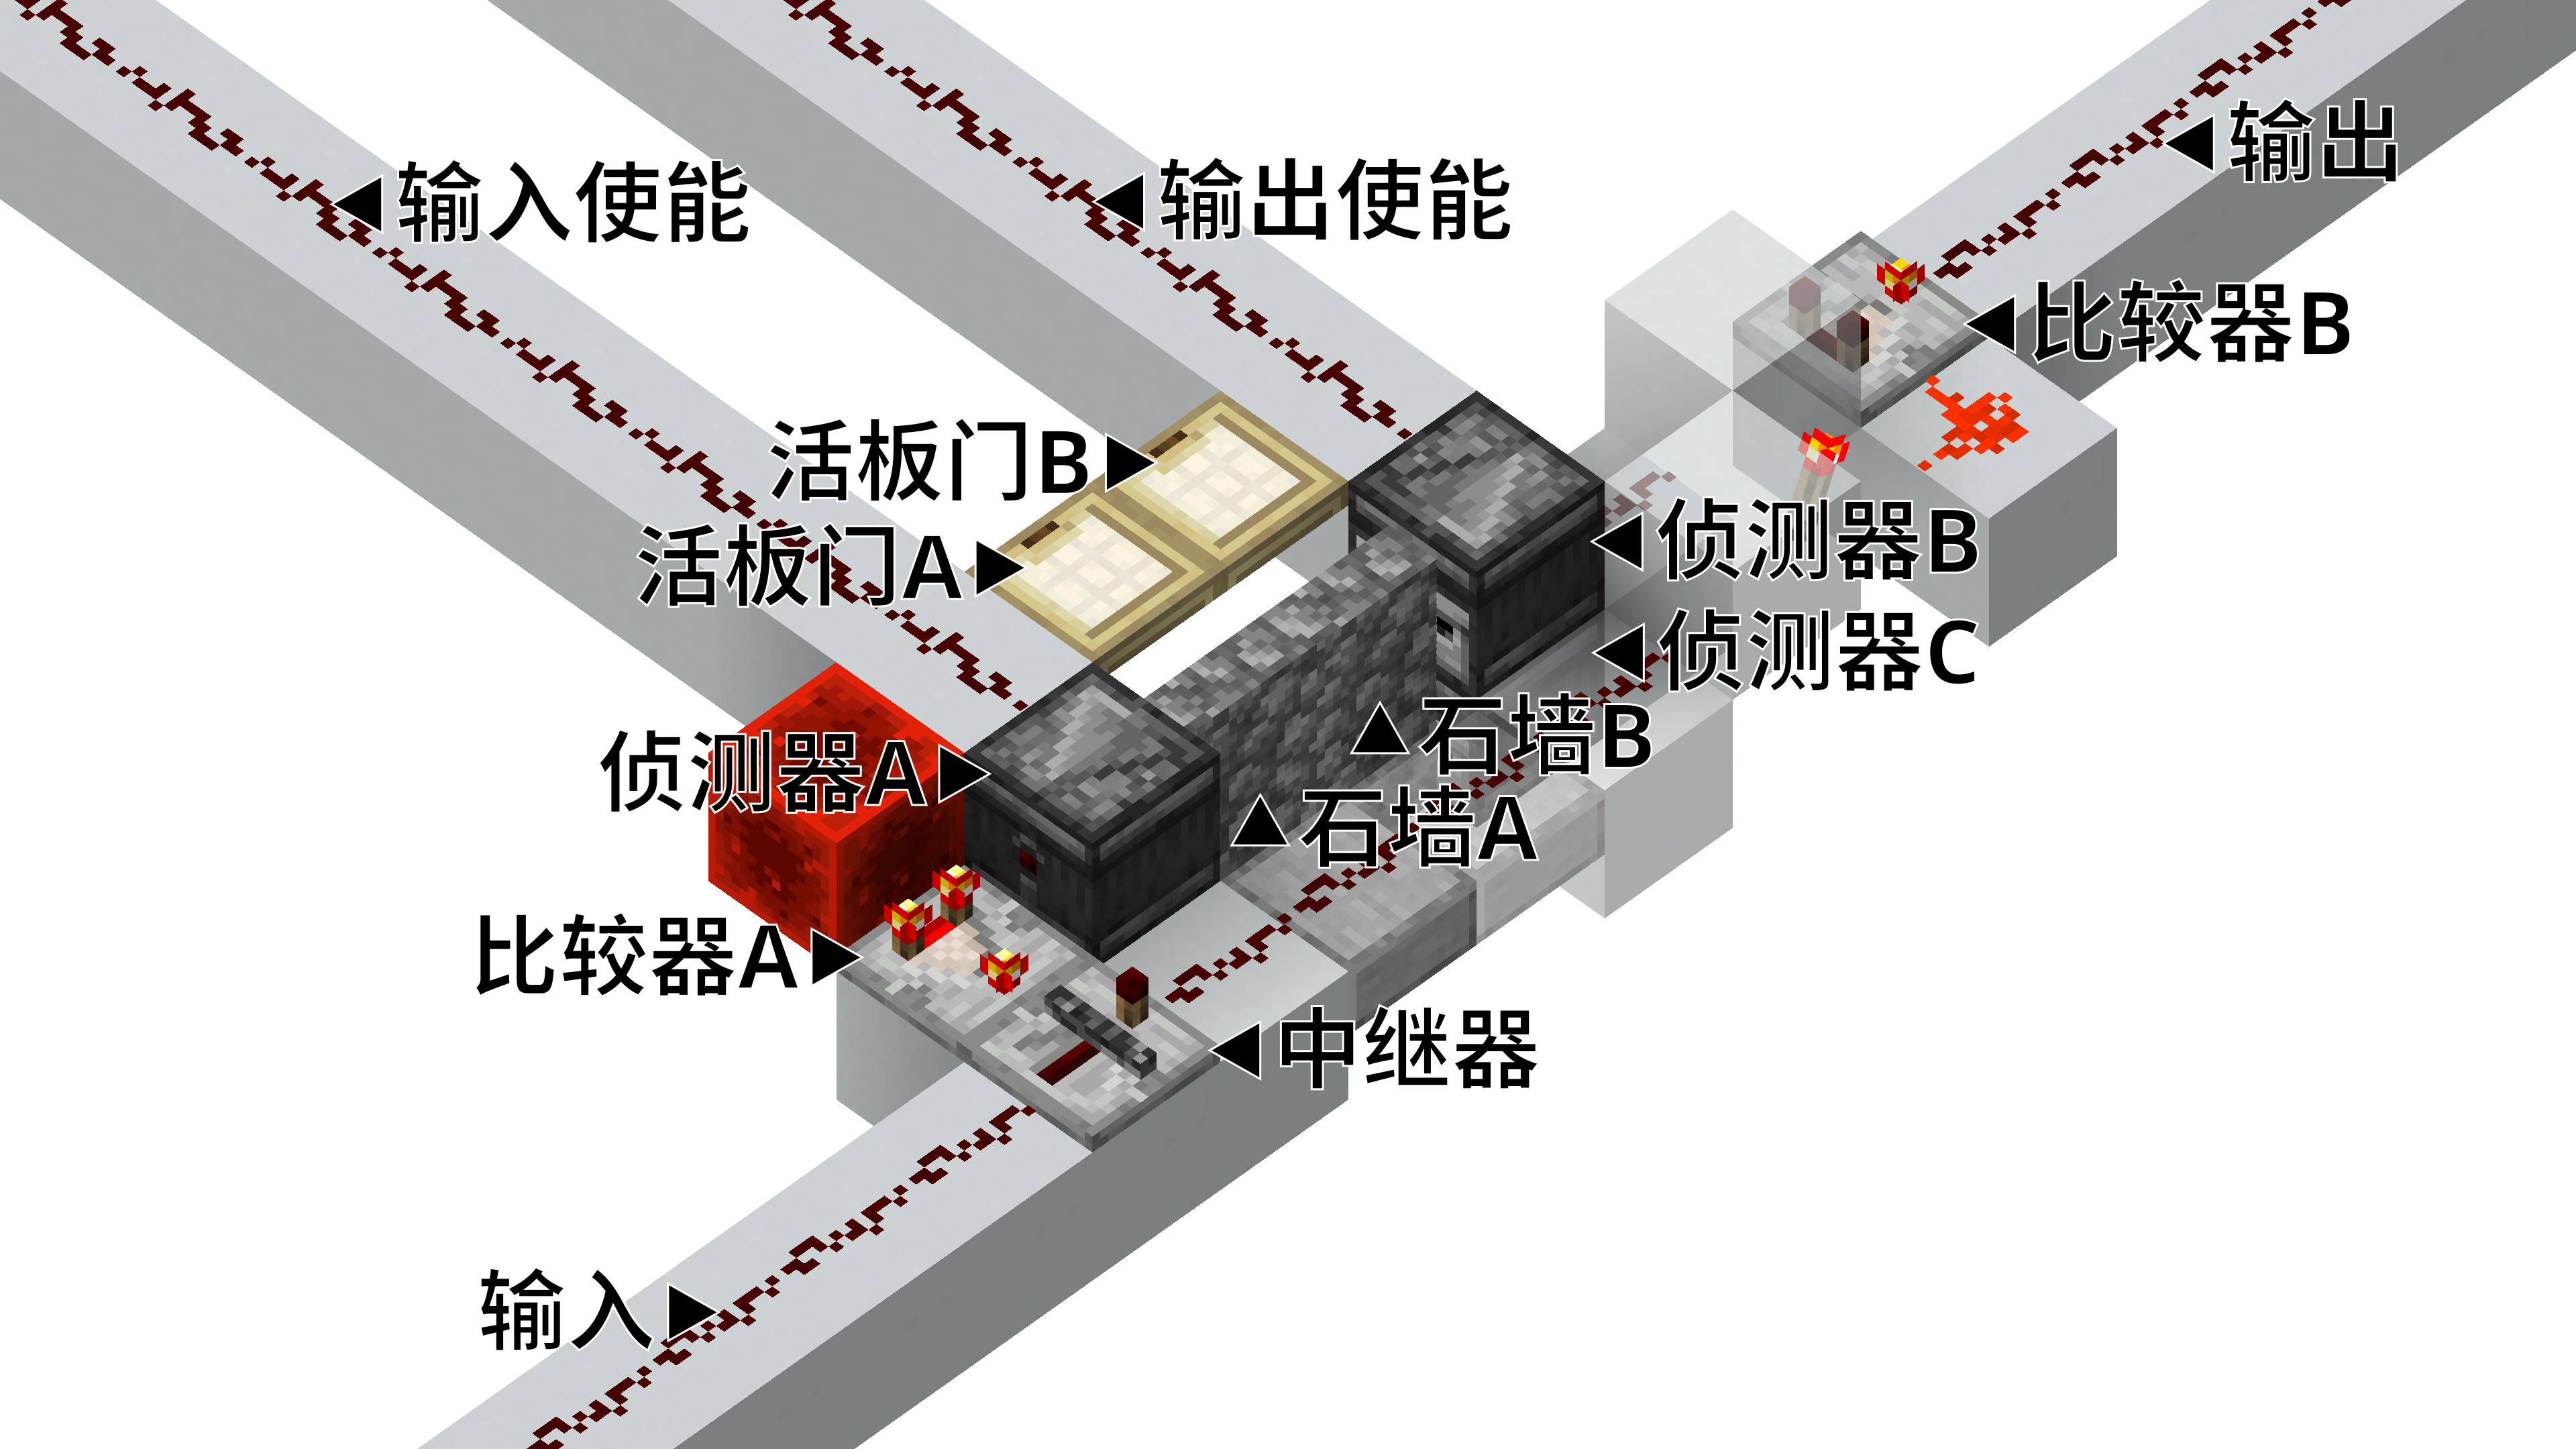
\includegraphics[width=0.75\linewidth]{figures/wall-based-storage.png}
        \caption{石墙存储器及标注}
        \label{fig:wall-based-storage-marked}
    \end{figure}

    \section{分析}
    在Minecraft中\footnote{本文所述内容均基于Minecraft: Java Edition 1.17.1版本, 但除石墙电路相关结论仅适用于Minecraft: Java Edition 1.16.x-1.17.x版本外\upcite{bib:wall}, 其他相关结论也应同样适用于Minecraft: Java Edition 1.13.x-1.17.x版本.\upcite{bib:tile-tick}}, 拥有延迟的红石元件(除活塞外)都会在接收到红石信号或方块更新时判断并为自己所在的方块位置添加(schedule, 也可译为安排)一个对应延迟后的计划刻(tile tick), 等计划刻被执行时再改变自身状态. 同一位置的方块在每个游戏刻内只能拥有一个计划刻, 重复安排的计划刻会被忽略. 在同一游戏刻内的计划刻先按照优先级(priority)数值从小到大的顺序依次执行, 优先级相同的计划刻再按照添加顺序执行. 需要注意的是, 计划刻并没有附加数据的功能. 红石元件执行计划刻时仅通过当前状态来判断要改变为的目标状态. 例如熄灭的中继器执行计划刻时就会亮起, 亮起的中继器执行计划刻时就会熄灭. 但比较器等元件(不包括中继器)在执行计划刻并改变状态前会先判断当前是否应该改变状态, 如果此时不满足改变状态的条件, 计划刻就会被忽略.\upcite{bib:tile-tick-component}\upcite{bib:yarn}

    \begin{figure}[tp!]
        \centering
        \begin{sequencediagram}
            \pgfumlsdunderlinefalse
            \newinst[0]{wire-input}{输入使能}{}
            \newinst[0]{door-a}{活板门A}{}
            \newinst[0]{wall-a}{石墙A}{}
            \newinst[0]{observer-a}{侦测器A}{}
            \newinst[0]{comparator-a}{比较器A}{}
            \newinst[0]{repeater}{中继器}{}
            \newinst[0]{wire-output}{存储信号}{}
            \newinst[1]{tile-tick}{计划刻系统}{}

            \timestamp{1游戏刻}

            \mess[0]{wire-input}{激活}{door-a}

            \highlightbegin{wire-input}

            \mess[0]{door-a}{使凸起}{wall-a}
            \mess[0]{wall-a}{更新}{observer-a}
            \mess[0]{observer-a}{添加计划刻}{tile-tick}

            \timestamp{2游戏刻}
            \timestamp{3游戏刻}

            \mess[0]{wire-input}{熄灭}{door-a}

            \highlightend{wire-input}

            \mess[0]{door-a}{使平整}{wall-a}
            \mess[0]{wall-a}{更新}{observer-a}
            \mess[0]{observer-a}{添加计划刻}{tile-tick}
            \mess[0]{tile-tick}{执行计划刻}{observer-a}
            \mess[0]{observer-a}{添加计划刻(重复添加, 失败)}{tile-tick}
            \mess[0]{observer-a}{侧面激活}{comparator-a}

            \highlightbegin{observer-a}

            \mess[0]{comparator-a}{添加计划刻(优先级为-1)*}{tile-tick}

            \timestamp{4游戏刻}
            \timestamp{5游戏刻}

            \mess[0]{tile-tick}{执行计划刻(优先级为-1)}{comparator-a}
            \mess[0]{comparator-a}{熄灭}{repeater}

            \highlightbegin{comparator-a}

            \mess[0]{repeater}{添加计划刻(优先级为-2)}{tile-tick}
            \mess[0]{tile-tick}{执行计划刻}{observer-a}
            \mess[0]{observer-a}{侧面熄灭}{comparator-a}

            \highlightend{observer-a}

            \mess[0]{comparator-a}{添加计划刻(优先级为-1)}{tile-tick}

            \timestamp{6游戏刻}
            \timestamp{7游戏刻}

            \mess[0]{tile-tick}{执行计划刻}{repeater}
            \mess[0]{repeater}{解锁}{wire-output}

            \highlightbegin{repeater}
            \highlightbegin{wire-output}

            \mess[0]{tile-tick}{执行计划刻}{comparator-a}
            \mess[0]{comparator-a}{激活}{repeater}

            \highlightend{comparator-a}

            \mess[0]{repeater}{添加计划刻(优先级为-2)}{tile-tick}

            \timestamp{8游戏刻}
            \timestamp{9游戏刻}

            \mess[0]{tile-tick}{执行计划刻}{repeater}
            \mess[0]{repeater}{锁存}{wire-output}

            \highlightend{repeater}
            \highlightend{wire-output}
        \end{sequencediagram}
        \caption{2游戏刻脉冲激活输入控制时钟信号线时各元件的微时序状态}
        \label{fig:micro-timing-sequence-input-2gt}
    \end{figure}

    \begin{figure}[tp!]
        \centering
        \begin{sequencediagram}
            \pgfumlsdunderlinefalse
            \newinst[0]{wire-input}{输出使能}{}
            \newinst[0]{door-b}{活板门B}{}
            \newinst[0]{wall-b}{石墙B}{}
            \newinst[0]{observer-b}{侦测器B}{}
            \newinst[0]{observer-c}{侦测器C}{}
            \newinst[0]{comparator-b}{比较器B}{}
            \newinst[0]{wire-output}{输出}{}
            \newinst[1]{tile-tick}{计划刻系统}{}

            \timestamp{1游戏刻}

            \mess[0]{wire-input}{激活}{door-a}

            \highlightbegin{wire-input}

            \mess[0]{door-b}{使凸起}{wall-b}
            \mess[0]{wall-b}{更新}{observer-b}
            \mess[0]{observer-b}{添加计划刻}{tile-tick}
            \mess[0]{wall-b}{更新}{observer-c}
            \mess[0]{observer-c}{添加计划刻}{tile-tick}

            \timestamp{2游戏刻}
            \timestamp{3游戏刻}

            \mess[0]{wire-input}{熄灭}{door-b}

            \highlightend{wire-input}

            \mess[0]{door-b}{使平整}{wall-b}
            \mess[0]{wall-b}{更新}{observer-b}
            \mess[0]{observer-b}{添加计划刻*}{tile-tick}
            \mess[0]{wall-b}{更新}{observer-c}
            \mess[0]{observer-c}{添加计划刻*}{tile-tick}
            \mess[0]{tile-tick}{执行计划刻}{observer-b}
            \mess[0]{observer-b}{添加计划刻(重复添加, 失败)}{tile-tick}
            \mess[0]{observer-b}{侧面激活}{comparator-b}

            \highlightbegin{observer-b}

            \mess[0]{comparator-b}{添加计划刻}{tile-tick}
            \mess[0]{tile-tick}{执行计划刻}{observer-c}
            \mess[0]{observer-c}{添加计划刻(重复添加, 失败)}{tile-tick}
            \mess[0]{observer-c}{侧面激活}{comparator-b}

            \highlightbegin{observer-c}

            \timestamp{4游戏刻}
            \timestamp{5游戏刻}
    
            \mess[0]{tile-tick}{执行计划刻}{observer-b}
            \mess[0]{observer-b}{侧面熄灭}{comparator-b}

            \highlightend{observer-b}
    
            \mess[0]{tile-tick}{执行计划刻}{observer-c}
            \mess[0]{observer-c}{侧面熄灭}{comparator-b}

            \highlightend{observer-c}

            \mess[0]{tile-tick}{执行计划刻(条件未满足, 失败)}{comparator-b}
        \end{sequencediagram}
        \caption{2游戏刻脉冲激活输出控制时钟信号线时各元件的微时序状态}
        \label{fig:micro-timing-sequence-output-2gt}
    \end{figure}

    \begin{figure}[tp!]
        \centering
        \begin{sequencediagram}
            \pgfumlsdunderlinefalse
            \newinst[0]{wire-input}{输出使能}{}
            \newinst[0]{door-b}{活板门B}{}
            \newinst[0]{wall-b}{石墙B}{}
            \newinst[0]{observer-b}{侦测器B}{}
            \newinst[0]{observer-c}{侦测器C}{}
            \newinst[0]{comparator-b}{比较器B}{}
            \newinst[0]{wire-output}{输出}{}
            \newinst[1]{tile-tick}{计划刻系统}{}

            \timestamp{1游戏刻}

            \mess[0]{wire-input}{激活}{door-a}

            \highlightbegin{wire-input}

            \mess[0]{door-b}{使凸起}{wall-b}
            \mess[0]{wall-b}{更新}{observer-b}
            \mess[0]{observer-b}{添加计划刻}{tile-tick}
            \mess[0]{wall-b}{更新}{observer-c}
            \mess[0]{observer-c}{添加计划刻}{tile-tick}

            \timestamp{2游戏刻}
            \timestamp{3游戏刻}

            \mess[0]{tile-tick}{执行计划刻}{observer-b}
            \mess[0]{observer-b}{添加计划刻*}{tile-tick}
            \mess[0]{observer-b}{激活}{comparator-b}

            \highlightbegin{observer-b}

            \mess[0]{comparator-b}{添加计划刻}{tile-tick}
            \mess[0]{tile-tick}{执行计划刻}{observer-c}
            \mess[0]{observer-c}{添加计划刻*}{tile-tick}
            \mess[0]{observer-c}{激活}{comparator-b}

            \highlightbegin{observer-c}

            \mess[0]{wire-input}{熄灭}{door-b}

            \highlightend{wire-input}

            \mess[0]{door-b}{使平整}{wall-b}
            \mess[0]{wall-b}{更新}{observer-b}
            \mess[0]{observer-b}{添加计划刻(重复添加, 失败)}{tile-tick}
            \mess[0]{wall-b}{更新}{observer-c}
            \mess[0]{observer-c}{添加计划刻(重复添加, 失败)}{tile-tick}

            \timestamp{4游戏刻}
            \timestamp{5游戏刻}
    
            \mess[0]{tile-tick}{执行计划刻}{observer-b}
            \mess[0]{observer-b}{熄灭}{comparator-b}

            \highlightend{observer-b}

            \mess[0]{tile-tick}{执行计划刻}{comparator-b}
            \mess[0]{comparator-b}{激活}{wire-output}

            \highlightbegin{comparator-b}
            \highlightbegin{wire-output}
    
            \mess[0]{tile-tick}{执行计划刻}{observer-c}
            \mess[0]{observer-c}{熄灭}{comparator-b}

            \highlightend{observer-c}

            \mess[0]{comparator-b}{添加计划刻}{tile-tick}

            \timestamp{6游戏刻}
            \timestamp{7游戏刻}

            \mess[0]{tile-tick}{执行计划刻}{comparator-b}
            \mess[0]{comparator-b}{熄灭}{wire-output}

            \highlightend{comparator-b}
            \highlightend{wire-output}
        \end{sequencediagram}
        \caption{延长的2游戏刻脉冲激活输出控制时钟信号线时各元件的微时序状态}
        \label{fig:micro-timing-sequence-output-longer-2gt}
    \end{figure}

    先对2游戏刻脉冲激活输入控制时钟信号线时的情况进行微时序分析, 如图\ref{fig:micro-timing-sequence-input-2gt}. 品红色线条代表元件被激活的时刻. 标有星号的一处微时序步骤是至关重要的. 在Minecraft中, 指向红石二极管(net.minecraft.block.AbstractRedstoneGateBlock类\upcite{bib:yarn}, 简称二极管,包括红石中继器和红石比较器)且该二极管非反向对顶的比较器遇到能量变化时, 会向自己添加优先级为-1的计划刻.\upcite{bib:tile-tick-component}\upcite{bib:yarn} 该计划刻会比优先级为0的侦测器A熄灭的计划刻更早执行, 因此在比较器A判断是否应该被激活时侦测器A尚未熄灭, 比较器A能够被从侧面激活(即被熄灭). 

    然而, 如图\ref{fig:micro-timing-sequence-output-2gt}对2游戏刻脉冲激活输出控制时钟信号线时的情况进行微时序分析, 可得知比较器B将不可能被激活. 比较器B并未指向二极管, 只能添加优先级为0的计划刻. 这个计划刻的添加时刻又晚于侦测器B和侦测器C的计划刻(标有星号的两处), 因此会在侦测器B和侦测器C的计划刻执行后(即熄灭后)再执行. 此时比较器B判断没有满足应该被激活的条件, 不能够被激活.

    在不延长脉冲至3游戏刻(即只使用延长的2游戏刻脉冲)的条件下能够使比较器B能被激活, 微时序分析如图\ref{fig:micro-timing-sequence-output-longer-2gt}. 比较器B虽然只能添加优先级为0的计划刻, 但这个计划刻的添加时刻恰好位于侦测器B和侦测器C的计划刻(标有星号的两处)之间, 因此会在侦测器B和侦测器C的计划刻之间执行. 此时侦测器B已经熄灭, 但侦测器C尚未熄灭, 比较器B满足应该被激活的条件, 能够被激活.
    
    \begin{figure}[t]
        \centering
        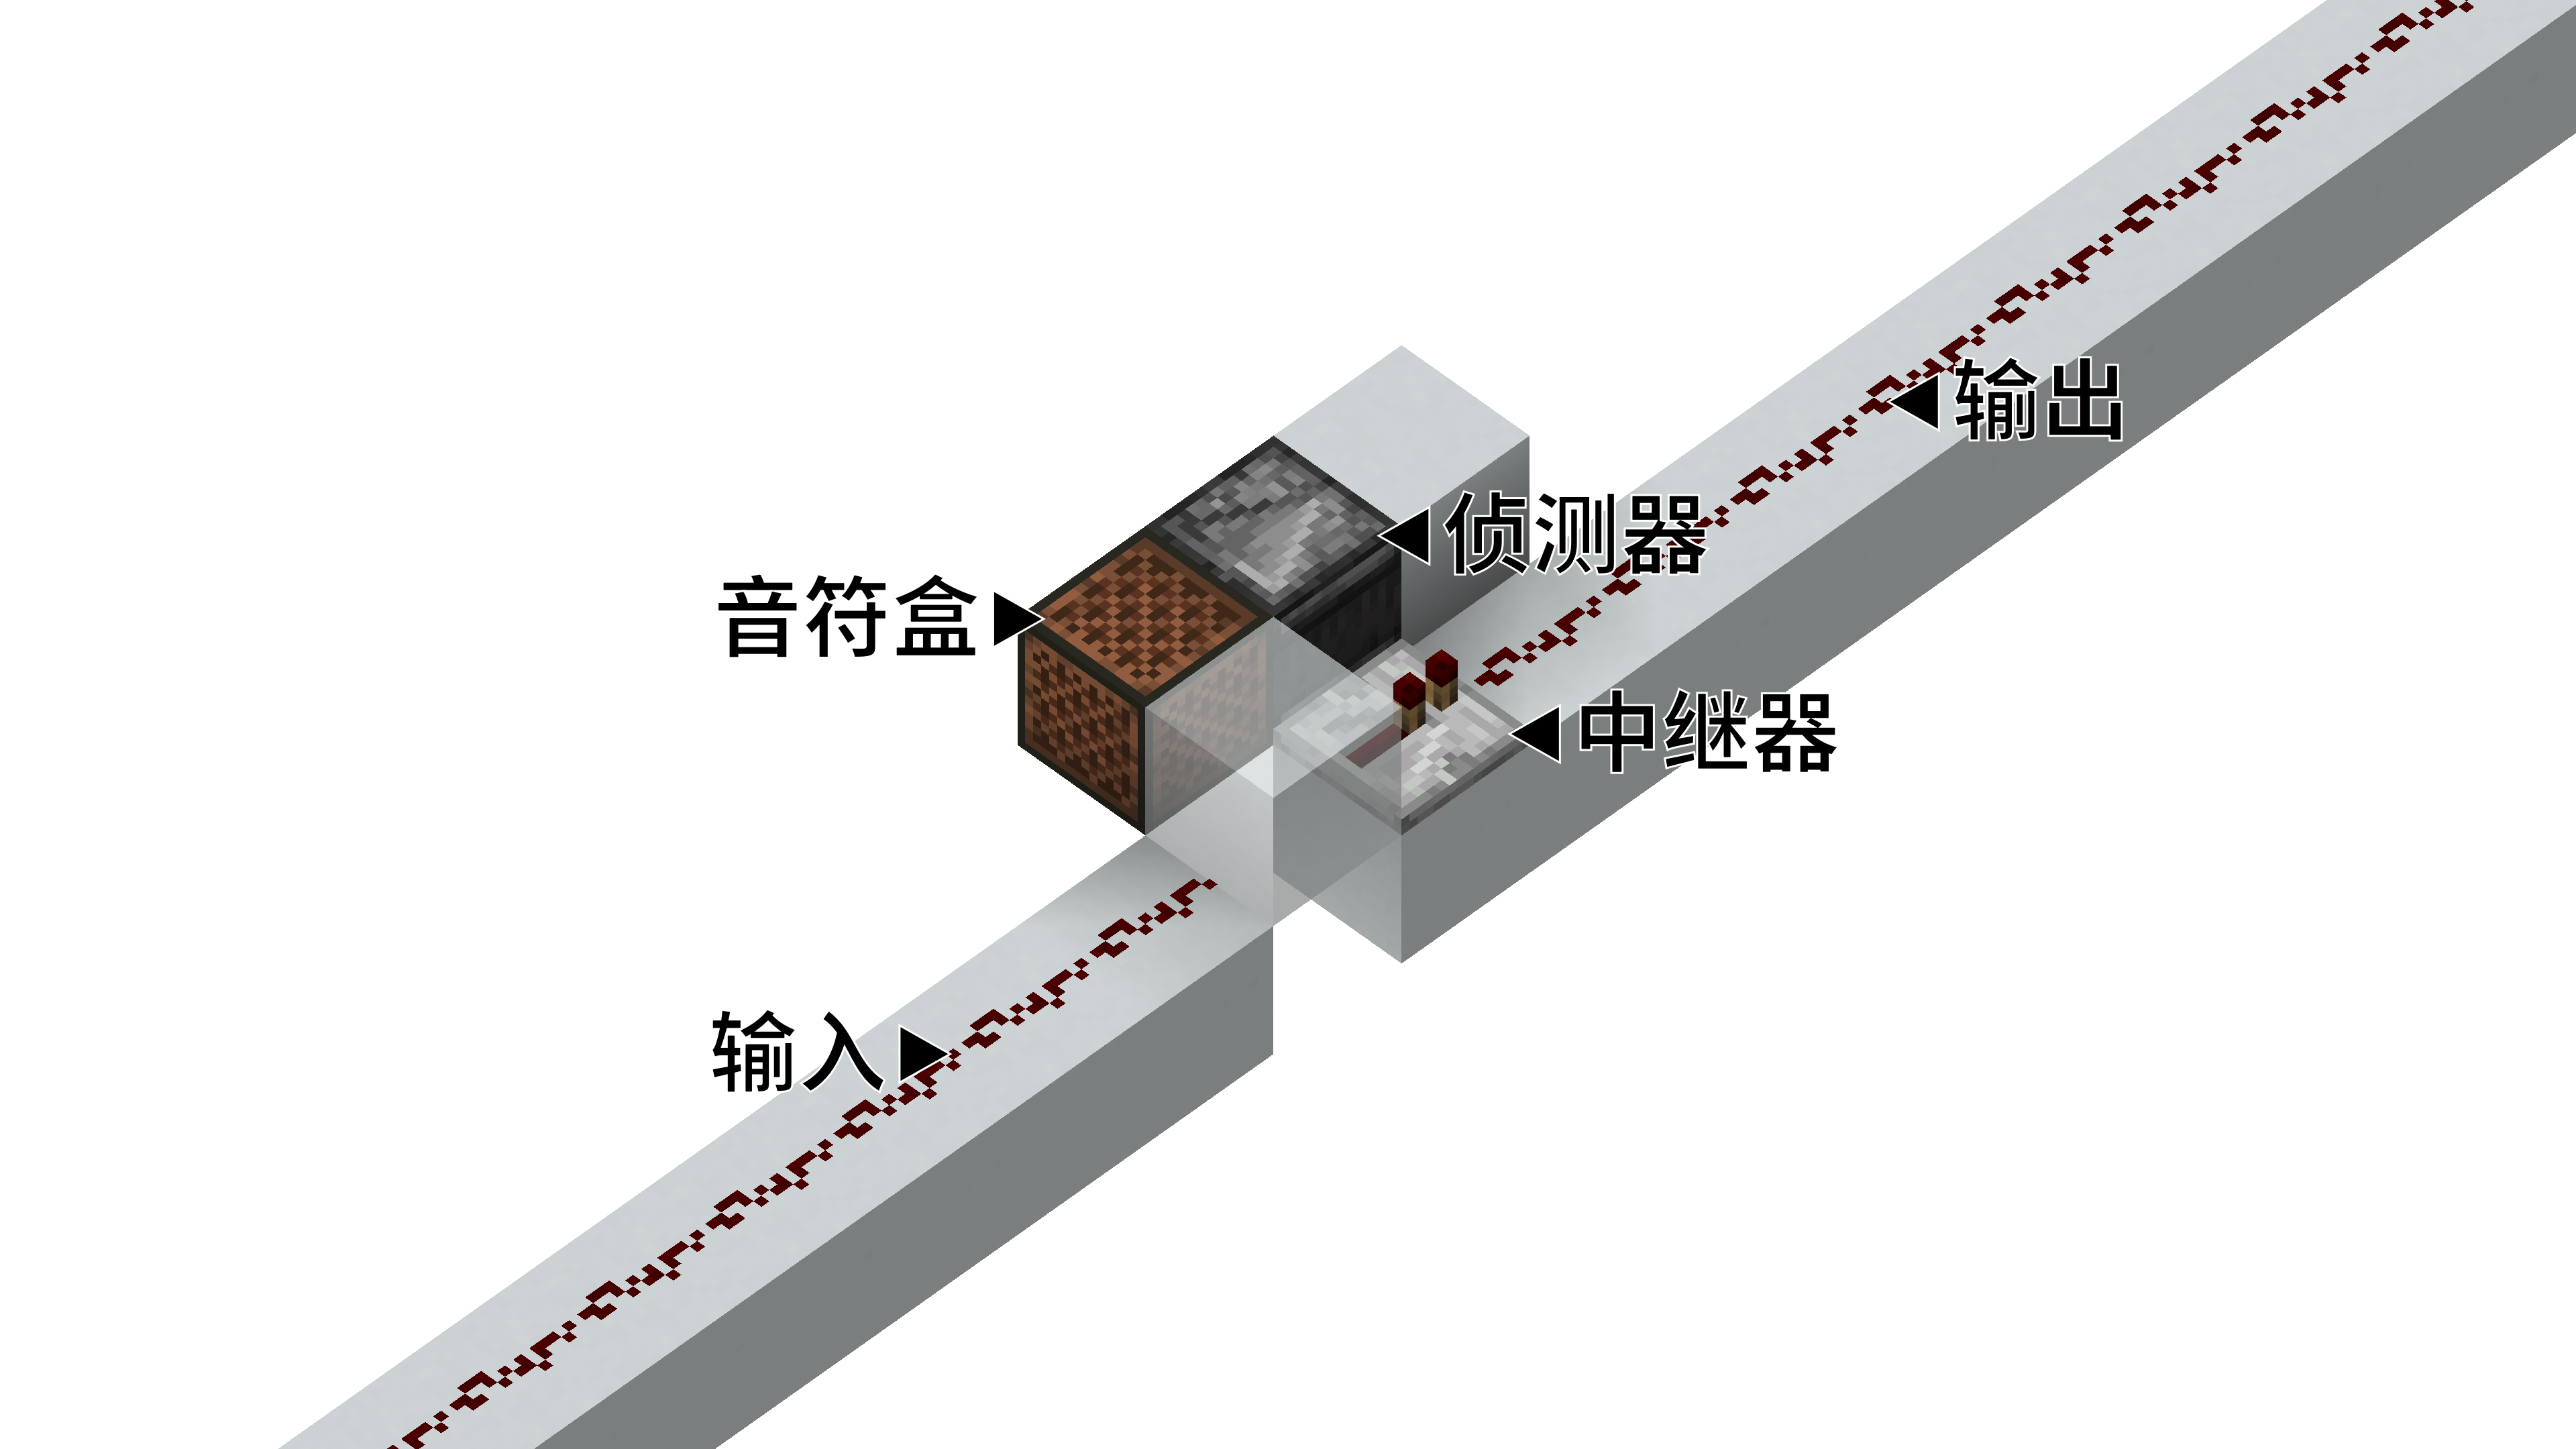
\includegraphics[width=0.75\linewidth]{figures/signal-extender.png}
        \caption{一种信号延长器的设计方案}
        \label{fig:signal-extender}
    \end{figure}

    \section{应用}
    延长2游戏刻脉冲的一种方法是使用如图\ref{fig:signal-extender}所示的利用了微时序特性的信号延长器. 该信号延长器的微时序分析如图\ref{fig:micro-timing-sequence-signal-extender-2gt}.
    
    需要注意的是, 这种信号延长器因为利用了中继器和侦测器计划刻优先级的差异, 不能延长经过了单独中继器的脉冲. 接受经过了单独中继器的2游戏刻脉冲时, 该信号延长器的微时序分析如图\ref{fig:micro-timing-sequence-signal-extender-shorter-2gt}. 这两种情况的关键区别在于输入信号熄灭的计划刻优先级不同, 导致了侦测器的计划刻与下游的计划刻(标有星号的两处)添加顺序不同, 接着导致了下游的计划刻执行时输出信号是否处于激活状态的差异, 最终导致下游计划刻执行成功或失败. 因此, 在使用图\ref{fig:wall-based-storage-marked}所示石墙存储器且必须使用2游戏刻脉冲激活输出时钟信号线时, 一种可行的方法是利用侦测器等计划刻优先级不低于0的元件生成脉冲并采用多个图\ref{fig:signal-extender}所示的信号延长器串联进行脉冲中继和延长.
    
    \begin{figure}[tp!]
        \centering
        \begin{sequencediagram}
            \pgfumlsdunderlinefalse
            \newinst[0]{wire-input}{输入}{}
            \newinst[0]{note-block}{音符盒}{}
            \newinst[0]{observer}{侦测器}{}
            \newinst[0]{repeater}{中继器}{}
            \newinst[0]{wire-output}{输出}{}
            \newinst[1]{tile-tick}{计划刻系统}{}

            \timestamp{1游戏刻}

            \mess[0]{wire-input}{激活}{repeater}

            \highlightbegin{wire-input}

            \mess[0]{repeater}{添加计划刻(优先级为-1)}{tile-tick}
            \mess[0]{wire-input}{激活}{note-block}
            \mess[0]{note-block}{更新}{observer}
            \mess[0]{observer}{添加计划刻}{tile-tick}

            \timestamp{2游戏刻}
            \timestamp{3游戏刻}

            \mess[0]{tile-tick}{执行计划刻}{repeater}
            \mess[0]{repeater}{添加计划刻(优先级为-2)}{tile-tick}
            \mess[0]{repeater}{激活}{wire-output}

            \highlightbegin{repeater}
            \highlightbegin{wire-output}

            \mess[0]{wire-output}{添加下游的计划刻*}{tile-tick}
            \mess[0]{wire-input}{熄灭}{repeater}
            \mess[0]{repeater}{添加计划刻(重复添加, 失败)}{tile-tick}
            \mess[0]{wire-input}{熄灭}{note-block}

            \highlightend{wire-input}

            \mess[0]{note-block}{更新}{observer}
            \mess[0]{observer}{添加计划刻*}{tile-tick}
            \mess[0]{tile-tick}{执行计划刻}{observer}
            \mess[0]{observer}{添加计划刻(重复添加, 失败)}{tile-tick}
            \mess[0]{observer}{激活}{wire-output}

            \highlightbegin{observer}

            \timestamp{4游戏刻}
            \timestamp{5游戏刻}
    
            \mess[0]{tile-tick}{执行计划刻}{repeater}
            \mess[0]{repeater}{熄灭}{wire-output}

            \highlightend{repeater}

            \mess[0]{tile-tick}{执行下游的计划刻}{wire-output}
    
            \mess[0]{tile-tick}{执行计划刻}{observer}
            \mess[0]{observer}{熄灭}{wire-output}

            \highlightend{observer}
            \highlightend{wire-output}
        \end{sequencediagram}
        \caption{信号延长器接受来自侦测器的2游戏刻脉冲时各元件的微时序状态}
        \label{fig:micro-timing-sequence-signal-extender-2gt}
    \end{figure}

    \begin{figure}[tp!]
        \centering
        \begin{sequencediagram}
            \pgfumlsdunderlinefalse
            \newinst[0]{wire-input}{输入}{}
            \newinst[0]{note-block}{音符盒}{}
            \newinst[0]{observer}{侦测器}{}
            \newinst[0]{repeater}{中继器}{}
            \newinst[0]{wire-output}{输出}{}
            \newinst[1]{tile-tick}{计划刻系统}{}

            \timestamp{1游戏刻}

            \mess[0]{wire-input}{激活}{repeater}

            \highlightbegin{wire-input}

            \mess[0]{repeater}{添加计划刻(优先级为-1)}{tile-tick}
            \mess[0]{wire-input}{激活}{note-block}
            \mess[0]{note-block}{更新}{observer}
            \mess[0]{observer}{添加计划刻}{tile-tick}

            \timestamp{2游戏刻}
            \timestamp{3游戏刻}

            \mess[0]{wire-input}{熄灭}{repeater}
            \mess[0]{repeater}{添加计划刻(优先级为-2)}{tile-tick}
            \mess[0]{wire-input}{熄灭}{note-block}

            \highlightend{wire-input}

            \mess[0]{note-block}{更新}{observer}
            \mess[0]{observer}{添加计划刻*}{tile-tick}
            \mess[0]{tile-tick}{执行计划刻}{repeater}
            \mess[0]{repeater}{添加计划刻(重复添加, 失败)}{tile-tick}
            \mess[0]{repeater}{激活}{wire-output}

            \highlightbegin{repeater}
            \highlightbegin{wire-output}

            \mess[0]{wire-output}{添加下游的计划刻*}{tile-tick}
            \mess[0]{tile-tick}{执行计划刻}{observer}
            \mess[0]{observer}{添加计划刻(重复添加, 失败)}{tile-tick}
            \mess[0]{observer}{激活}{wire-output}

            \highlightbegin{observer}

            \timestamp{4游戏刻}
            \timestamp{5游戏刻}
    
            \mess[0]{tile-tick}{执行计划刻}{repeater}
            \mess[0]{repeater}{熄灭}{wire-output}

            \highlightend{repeater}
    
            \mess[0]{tile-tick}{执行计划刻}{observer}
            \mess[0]{observer}{熄灭}{wire-output}

            \highlightend{observer}
            \highlightend{wire-output}

            \mess[0]{tile-tick}{执行下游的计划刻(失败)}{wire-output}
        \end{sequencediagram}
        \caption{信号延长器接受经过了单独中继器的2游戏刻脉冲时各元件的微时序状态}
        \label{fig:micro-timing-sequence-signal-extender-shorter-2gt}
    \end{figure}
    
    \section{结语}
    图\ref{fig:wall-based-storage-marked}所示石墙存储器在减少时延的同时因使用了微时序特性而带来了不稳定性. 而这种不稳定性可以通过进一步利用微时序特性来消除. 合理运用微时序特性能在一些方面有效提高红石装置的性能, 许多微时序特性也是多版本通用的. 微时序不只是令人感到疑惑的一种特性, 也能在某些领域发挥它的作用.
    
    \renewcommand{\refname}{主要参考文献}
    \begin{thebibliography}{99}
        \bibitem{bib:wall-based-storage}辰占鳌头. 基于石墙电路的随机存储器[J/OL]. 红石数电评论, 2021, 10.
        \bibitem{bib:wall}森森. 关于“墙”在Minecraft红石数字电路中的应用[J/OL]. 红色的粉末, 2020. \url{https://zhuanlan.zhihu.com/p/375262793}.
        \bibitem{bib:tile-tick}Fallen\_Breath. 计划刻[J/OL]. 深度剖析Minecraft, 2020, 3. \url{https://fallenbreath.me/2020/09/16/deeply-dissecting-minecraft_3/}.
        \bibitem{bib:tile-tick-component}Fallen\_Breath. 计划刻元件[J/OL]. 深度剖析Minecraft, 2020, 3.4. \url{https://fallenbreath.me/2020/09/17/deeply-dissecting-minecraft_3.4/}.
        \bibitem{bib:yarn}yarn[CP/OL]. 版本1.17.1+build.63. \url{https://github.com/FabricMC/yarn/actions/runs/3974649221}.
    \end{thebibliography}
\end{document}